% =============================================================================
% SLIDE: WHY TOPOLOGICAL SORTING FOR DAG TASK SCHEDULING
% =============================================================================
% Removed per request: Why Topological Sorting is Chosen for DAG Task Scheduling.
\iffalse
\begin{frame}[t]{Why Topological Sorting is Chosen for DAG Task Scheduling}
\vspace{-0.55em}

% Top Concept Pillars (3 Columns)
\begin{columns}[T]
\begin{column}{0.32\textwidth}
  \begin{tcolorbox}[
    enhanced, arc=2.5pt, colframe=lavenderDark!85, colback=lavenderLight!35,
    title={\scriptsize\bfseries\color{white}\faProjectDiagram\; 1. Task Dependencies},
    boxrule=0.55pt, left=3pt, right=3pt, top=1.2pt, bottom=1.2pt
  ]
  \fontsize{4.6}{5.5}\selectfont
  $\bullet$\;\textbf{Prerequisites first:} A task starts after the tasks it needs are finished.\\
  $\bullet$\;\textbf{Independent work:} Unrelated tasks can run in any order.
  \end{tcolorbox}
\end{column}

\begin{column}{0.34\textwidth}
  \begin{tcolorbox}[
    enhanced, arc=2.5pt, colframe=prismTeal!85!black, colback=prismMint!35,
    title={\scriptsize\bfseries\color{white}\faExclamationTriangle\; 2. Finds Waiting Loops},
    boxrule=0.55pt, left=3pt, right=3pt, top=1.2pt, bottom=1.2pt
  ]
  \fontsize{4.6}{5.5}\selectfont
  $\bullet$\;\textbf{Finds circular waiting:} Detects loops such as $A$ waits for $B$, while $B$ waits for $A$.\\
  $\bullet$\;\textbf{Stops safely:} Reports the problem instead of waiting forever.
  \end{tcolorbox}
\end{column}

\begin{column}{0.32\textwidth}
  \begin{tcolorbox}[
    enhanced, arc=2.5pt, colframe=lavenderMedium!90, colback=lavenderLight!35,
    title={\scriptsize\bfseries\color{white}\faCogs\; 3. Runs Work in Parallel},
    boxrule=0.55pt, left=3pt, right=3pt, top=1.2pt, bottom=1.2pt
  ]
  \fontsize{4.6}{5.5}\selectfont
  $\bullet$\;\textbf{Ready tasks:} Tasks with no unfinished prerequisites can start together.\\
  $\bullet$\;\textbf{Safe hand-off:} The next task starts only when all required inputs arrive.
  \end{tcolorbox}
\end{column}
\end{columns}

\vspace{-0.45em}

% Comparative Analysis Table
\begin{tcolorbox}[
  enhanced, arc=3pt, colframe=lavenderDark!75, colback=white,
  boxrule=0.55pt, left=2.0pt, right=2.0pt, top=0.8pt, bottom=0.8pt, width=\linewidth,
  title={\scriptsize\bfseries\color{white}\faTable\; Simple Comparison: Topological Sort vs. Common Sorting}
]
\setlength{\tabcolsep}{2.2pt}
\fontsize{4.2}{5.1}\selectfont
\renewcommand{\arraystretch}{1.03}
\begin{tabularx}{\linewidth}{>{\raggedright\arraybackslash}m{2.30cm} | >{\centering\arraybackslash}m{1.80cm} | >{\raggedright\arraybackslash}m{2.50cm} | >{\centering\arraybackslash}m{1.40cm} | >{\centering\arraybackslash}m{1.45cm} | >{\centering\arraybackslash}m{1.50cm} | >{\raggedright\arraybackslash}X}
\hline
\rowcolor{lavenderLight!90}
\textbf{Method} & \textbf{Works With} & \textbf{How It Orders} & \textbf{Speed} & \textbf{Finds Loops} & \textbf{Parallel Work} & \textbf{Useful for Task Workflows} \\
\hline

\rowcolor{prismMint!85}
\textbf{\color{prismTeal!90!black}\faCheckCircle\; Topological Sort} &
Task dependency graph &
\textbf{Prerequisites first} &
$\mathcal{O}(V + E)$ &
{\color{prismTeal!90!black}\textbf{Yes}} (In-degree) &
{\color{prismTeal!90!black}\textbf{Yes}} (Fan-out) &
\textbf{\color{prismTeal!90!black}Best choice:} Follows task dependencies and runs independent tasks together. \\
\hline

\textbf{Merge Sort} &
List of values &
\textbf{Smallest value first} &
$\mathcal{O}(n \log n)$ &
{\color{red!75!black}\faTimesCircle\; No} (N/A) &
{\color{red!75!black}\faTimesCircle\; No} (Serial 1D) &
{\color{red!75!black}\textbf{Not suitable:}} Sorts values, not task prerequisites. \\
\hline

\textbf{Quick Sort} &
List of values &
\textbf{Around a pivot value} &
$\mathcal{O}(n \log n)$ avg &
{\color{red!75!black}\faTimesCircle\; No} (N/A) &
{\color{red!75!black}\faTimesCircle\; No} (Serial 1D) &
{\color{red!75!black}\textbf{Not suitable:}} Does not know which task must come first. \\
\hline

\textbf{Heap Sort} &
Priority list &
\textbf{Highest priority first} &
$\mathcal{O}(n \log n)$ &
{\color{red!75!black}\faTimesCircle\; No} (N/A) &
{\color{red!75!black}\faTimesCircle\; No} (Serial 1D) &
{\color{red!75!black}\textbf{Not suitable:}} Priority alone cannot enforce several prerequisites. \\
\hline

\textbf{Bubble / Insertion} &
List of values &
\textbf{Neighbor comparisons} &
$\mathcal{O}(n^2)$ &
{\color{red!75!black}\faTimesCircle\; No} (N/A) &
{\color{red!75!black}\faTimesCircle\; No} (Strict Serial) &
{\color{red!75!black}\textbf{Not suitable:}} Pairwise swaps cannot represent task dependencies. \\
\hline
\end{tabularx}
\end{tcolorbox}

\vspace{-0.42em}
\begin{tcolorbox}[
  enhanced, arc=2.5pt, colframe=prismTeal!75, colback=prismMint!30,
  boxrule=0.45pt, left=3.5pt, right=3.5pt, top=1.0pt, bottom=1.0pt
]
\fontsize{4.3}{5.1}\selectfont\color{lavenderDark}
\textbf{Why This Matters for PrismSpace:} Regular sorting puts numbers or words in order. PrismSpace must order tasks based on their prerequisites. \textbf{Topological sorting} follows those prerequisites, detects circular dependencies, and lets independent tasks run together.
\end{tcolorbox}

\end{frame}
\fi

% =============================================================================
% SLIDE: PROVIDER ROUTING
% =============================================================================
\providecolor{groqOrange}{RGB}{245, 79, 53}
\providecolor{openaiGreen}{RGB}{16, 163, 127}
\providecolor{nvidiaGreen}{RGB}{118, 185, 0}

\iffalse
\begin{frame}[t]{Agent \& Provider Router working}
\vspace{-0.78em}

% Top Concept Banner: Technically Simplified Goal
\begin{tcolorbox}[
  enhanced, arc=2.5pt, colframe=lavenderDark!90, colback=lavenderLight!40,
  boxrule=0.55pt, left=4pt, right=4pt, top=1.0pt, bottom=1.0pt
]
\fontsize{4.7}{5.6}\selectfont
\textbf{\color{lavenderDark}\faRoute\; Core Routing Mission:}\quad
Instead of sending every query to a slow, expensive frontier model, PrismSpace dynamically routes each agent sub-task to the \textbf{fastest, most cost-effective provider} that clears the task's required \textbf{quality threshold ($\tau$)}.
\end{tcolorbox}

\vspace{-0.44em}

% Pipeline Diagram Container
\begin{tcolorbox}[
  enhanced, arc=3pt, colframe=lavenderDark!80, colback=white,
  title={\scriptsize\bfseries\color{white}\faSlidersH\; End-to-End Provider Routing Pipeline},
  boxrule=0.6pt, left=2.0pt, right=2.0pt, top=0.9pt, bottom=0.9pt
]
\centering
\adjustbox{max width=0.99\linewidth, max totalheight=0.47\textheight, keepaspectratio}{%
\begin{tikzpicture}[
  node distance=0.25cm,
  stepnode/.style={
    rectangle, rounded corners=3.5pt, draw=lavenderDark!75, fill=lavenderLight!50,
    minimum height=1.54cm, text width=2.15cm, align=center, inner sep=2.5pt,
    font=\fontsize{5.2}{6.2}\selectfont
  },
  poolnode/.style={
    rectangle, rounded corners=3.5pt, draw=prismTeal!80!black, fill=prismMint!35,
    minimum height=1.54cm, text width=4.35cm, align=center, inner sep=2.0pt
  },
  filternode/.style={
    rectangle, rounded corners=3.5pt, draw=prismBlue!85!black, fill=lavenderLight!65,
    minimum height=1.54cm, text width=2.15cm, align=center, inner sep=2.5pt,
    font=\fontsize{5.2}{6.2}\selectfont
  },
  scorenode/.style={
    rectangle, rounded corners=3.5pt, draw=prismTeal!85!black, fill=prismMint!60,
    minimum height=1.54cm, text width=2.20cm, align=center, inner sep=2.5pt,
    font=\fontsize{5.2}{6.2}\selectfont
  },
  dispatchnode/.style={
    rectangle, rounded corners=3.5pt, draw=lavenderDark!90, fill=lavenderLight!80,
    minimum height=1.54cm, text width=2.20cm, align=center, inner sep=2.5pt,
    font=\fontsize{5.2}{6.2}\selectfont
  },
  parr/.style={-{Stealth[scale=0.70]}, line width=0.90pt, draw=lavenderDark!90!black,
    shorten <=0.02cm, shorten >=0.02cm}
]

  % 1. Task Profile
  \node[stepnode] (step1) at (0, 0) {
    \textbf{\color{lavenderDark}\faTasks\; 1. Task Profile}\\[1.5pt]
    \fontsize{4.5}{5.4}\selectfont
    \textbf{Input:} User task + constraints\\
    \textbf{Working:} Extract task type, quality needs, privacy, and deadline\\
    \textbf{Output:} Routing requirements
  };

  % 2. Candidate Pool with Real Logos
  \node[poolnode] (step2) at (4.10, 0) {
    {\fontsize{5.2}{6.2}\selectfont\textbf{\color{prismTeal!90!black}\faServer\; 2. Candidate Pool}}\\[-1pt]
    {\fontsize{4.4}{5.2}\selectfont\textbf{Input:} routing requirements \quad | \quad \textbf{Working:} check provider capabilities \quad | \quad \textbf{Output:} candidate models}\\[1pt]
    % Groq Card
    \begin{tcolorbox}[
      enhanced, arc=2pt, colframe=groqOrange!85, colback=white,
      boxrule=0.45pt, left=1.5pt, right=1.5pt, top=0.6pt, bottom=0.6pt, width=4.20cm
    ]
      \begin{minipage}[c]{0.11\linewidth}
        \centering
\includegraphics[height=0.28cm,keepaspectratio]{logos/groq.png}
      \end{minipage}%
      \begin{minipage}[c]{0.87\linewidth}
        \fontsize{4.5}{5.4}\selectfont
        \textbf{\color{groqOrange!95!black}Groq LPU:} Blazing speed ($\approx 500$ tok/s, lowest cost)\\
        \textit{Role: Fast streaming, tool calls \& instant summaries}
      \end{minipage}
    \end{tcolorbox}
    \vspace{-0.24cm}
    % OpenAI Card
    \begin{tcolorbox}[
      enhanced, arc=2pt, colframe=openaiGreen!85, colback=white,
      boxrule=0.45pt, left=1.5pt, right=1.5pt, top=0.6pt, bottom=0.6pt, width=4.20cm
    ]
      \begin{minipage}[c]{0.11\linewidth}
        \centering
\includegraphics[height=0.28cm,keepaspectratio]{logos/openai.png}
      \end{minipage}%
      \begin{minipage}[c]{0.87\linewidth}
        \fontsize{4.5}{5.4}\selectfont
        \textbf{\color{openaiGreen!95!black}OpenAI GPT-4o:} Frontier IQ \& deep reasoning\\
        \textit{Role: Complex planning, code synthesis \& math logic}
      \end{minipage}
    \end{tcolorbox}
    \vspace{-0.24cm}
    % NVIDIA NIM Card
    \begin{tcolorbox}[
      enhanced, arc=2pt, colframe=nvidiaGreen!85, colback=white,
      boxrule=0.45pt, left=1.5pt, right=1.5pt, top=0.6pt, bottom=0.6pt, width=4.20cm
    ]
      \begin{minipage}[c]{0.11\linewidth}
        \centering
\includegraphics[height=0.28cm,keepaspectratio]{logos/nvidia.png}
      \end{minipage}%
      \begin{minipage}[c]{0.87\linewidth}
        \fontsize{4.5}{5.4}\selectfont
        \textbf{\color{nvidiaGreen!95!black}NVIDIA NIM:} Self-hosted / Open Llama-3 70B\\
        \textit{Role: Enterprise microservice, private zero-leak GPU}
      \end{minipage}
    \end{tcolorbox}
  };

  % 3. Filter
  \node[filternode] (step3) at (8.20, 0) {
    \textbf{\color{prismBlue!90!black}\faFilter\; 3. Hard Filter}\\[1.5pt]
    \fontsize{4.5}{5.4}\selectfont
    \textbf{Input:} candidate models\\[-1pt]
    \textbf{Working:} remove models that cannot satisfy the task\\[-1pt]
    \textbf{Checks:} context, availability, privacy\\[-1pt]
    \textbf{Output:} eligible models
  };

  % 4. Score
  \node[scorenode] (step4) at (11.25, 0) {
    \textbf{\color{prismTeal!90!black}\faBalanceScale\; 4. Smart Scoring}\\[1.5pt]
    \fontsize{4.5}{5.4}\selectfont
    \textbf{Input:} eligible models\\[-1pt]
    \textbf{Algorithm:} XGBoost ranking/classifier\\[-1pt]
    \textbf{Working:} compare task needs with model capabilities\\[-1pt]
    \textbf{Output:} ranked model list
  };

  % 5. Dispatch
  \node[dispatchnode] (step5) at (14.30, 0) {
    \textbf{\color{lavenderDark}\faPaperPlane\; 5. Dispatch \& Fallback}\\[1.5pt]
    \fontsize{4.5}{5.4}\selectfont
    \textbf{Input:} selected model + task\\[-1pt]
    \textbf{Working:} send request, monitor execution, and use fallback if needed\\[-1pt]
    \textbf{Output:} model response + telemetry\\[-1pt]
    \textbf{Result:} tool/API response
  };

  % Place each hand-off label above its arrow, centered in the gap between boxes.
  \tikzset{flowlabel/.style={midway, above=1.5pt, fill=white, inner sep=0.6pt,
    text width=0.58cm, align=center,
    font=\fontsize{3.8}{4.3}\selectfont\bfseries, text=lavenderDark}}
  \draw[parr] (step1.east) -- node[flowlabel] {Output:\\ \{task\_profile\}} (step2.west);
  \draw[parr] (step2.east) -- node[flowlabel] {Output:\\ \{candidates[]\}} (step3.west);
  \draw[parr] (step3.east) -- node[flowlabel] {Output:\\ \{eligible[]\}} (step4.west);
  \draw[parr] (step4.east) -- node[flowlabel] {Output:\\ \{selected\_model\}} (step5.west);

\end{tikzpicture}%
}
\end{tcolorbox}

\vspace{0.38em}

% Bottom Full-Width Decision Rule
\begin{tcolorbox}[
  enhanced, arc=2.5pt, colframe=prismTeal!80!black, colback=prismMint!35,
  title={\scriptsize\bfseries\color{white}\faCalculator\; How the Router Decides (Multi-Objective Optimization)},
  boxrule=0.52pt, left=3.5pt, right=3.5pt, top=0.7pt, bottom=0.7pt,
  height=1.25cm, valign=center
]
\fontsize{4.3}{5.2}\selectfont
\raggedright
$\bullet$\;\textbf{Speed-Critical Nodes ($\lambda_l \uparrow$):} Fast tool calls prioritize low latency $\rightarrow$ routes to \textbf{Groq LPU} ($<300\text{ms}$).\\[1.6pt]
$\bullet$\;\textbf{High-Complexity Tasks ($\tau \uparrow$):} Architectural synthesis prioritizes IQ $\rightarrow$ routes to \textbf{OpenAI GPT-4o}.\\[1.6pt]
$\bullet$\;\textbf{Confidential Workflows:} Data protection requirements lock execution to local \textbf{NVIDIA NIM} microservices.
\end{tcolorbox}
\end{frame}
\fi

% Rebuilt provider-routing diagram: coherent data flow with explicit payloads.
\begin{frame}[t]{Agent \& Provider Router working}
\vspace{-0.62em}

\begin{tcolorbox}[
  enhanced, arc=2.5pt, colframe=lavenderDark!90, colback=lavenderLight!40,
  boxrule=0.55pt, left=5pt, right=5pt, top=1.5pt, bottom=1.5pt
]
\fontsize{5.0}{6.0}\selectfont
\textbf{Routing goal:} Convert a task profile into one suitable model request, then return the model response.
\end{tcolorbox}

\vspace{0.10em}
\centering
\begin{adjustbox}{max width=1.04\linewidth, max totalheight=0.74\textheight, keepaspectratio}
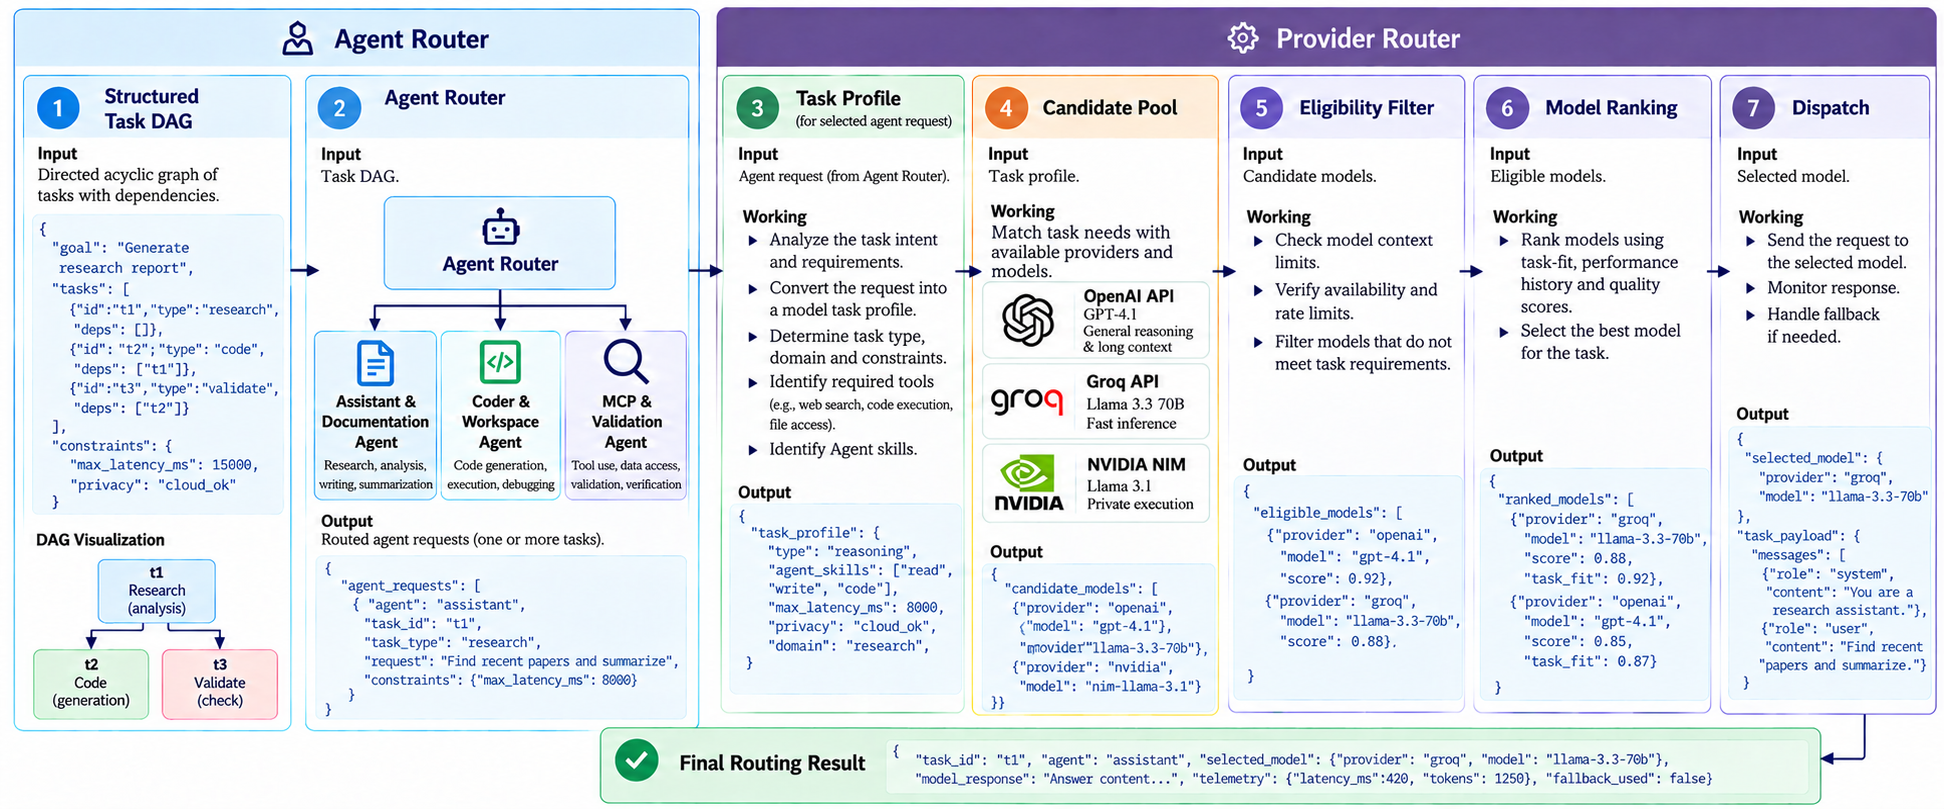
\includegraphics[width=1.04\linewidth, trim=8 6 8 6, clip]{AgentandProviderRouting-Pipeline.png}
\end{adjustbox}
\end{frame}

% =============================================================================
% SLIDE: ORPO
% =============================================================================
\begin{frame}[t]{How ORPO Works: Preference Alignment and Quality Gating}
\vspace{-0.80em}

% Top Concept Banner: What is ORPO & Why as a Reward System?
\begin{tcolorbox}[
  enhanced, arc=2.5pt, colframe=lavenderDark!90, colback=lavenderLight!45,
  boxrule=0.55pt, left=4pt, right=4pt, top=1.8pt, bottom=1.8pt
]
\fontsize{4.8}{5.8}\selectfont
\textbf{\color{lavenderDark}\faBalanceScale\; What is ORPO \& Why is it Used Here as a Reward System?}\\[0.5pt]
$\bullet$\;\textbf{What is ORPO?} \textbf{Odds Ratio Preference Optimization (ORPO)} is an integrated \textbf{single-stage reward and alignment algorithm}. Traditional \textbf{Reinforcement Learning from Human Feedback (RLHF)} requires training a separate reward model and keeping a frozen reference model in GPU memory (heavy, slow, and unstable).\\
$\bullet$\;\textbf{Why in PrismSpace?} In multi-agent swarms, LLMs can hallucinate invalid tools or malformed code. ORPO acts as an \textbf{internal reward filter}: it mathematically rewards compliant trajectories ($y_w$) and penalizes bad responses ($y_l$) during fine-tuning, eliminating the need for an external reward model.
\end{tcolorbox}

\vspace{-0.55em}

% Interactive & Intuitive Workflow Diagram
\centering\vspace{-0.10em}
\adjustbox{max width=0.99\linewidth, max totalheight=0.69\textheight, keepaspectratio}{%
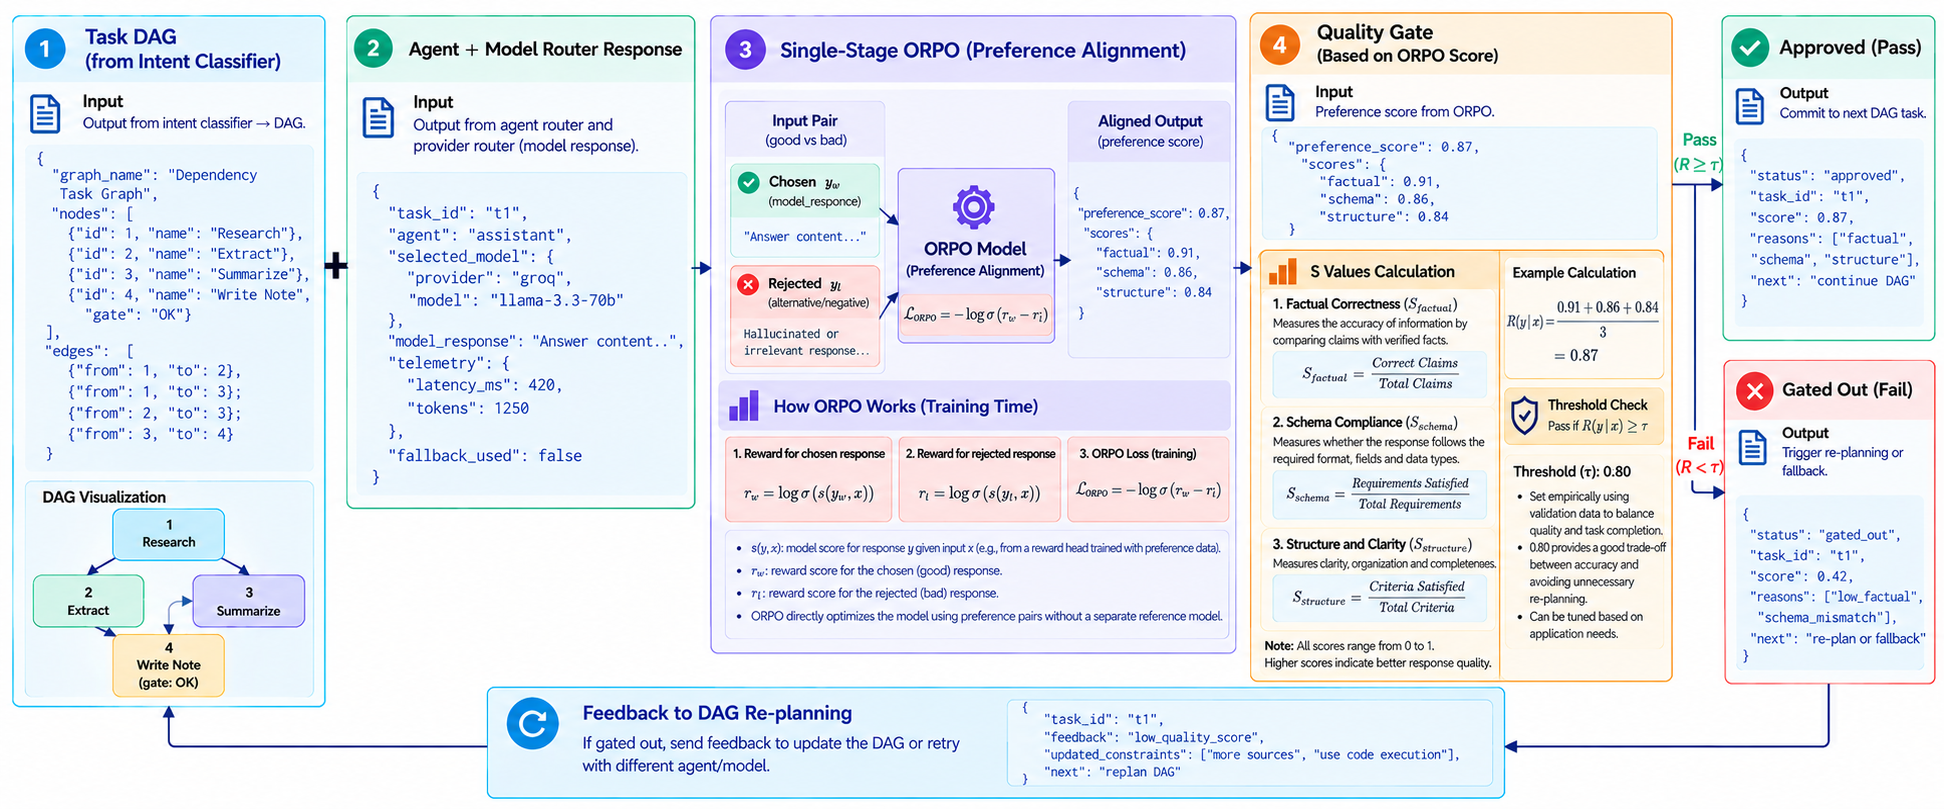
\includegraphics[width=0.99\linewidth, trim=0 10 0 10, clip]{ORPO.png}%
}
\end{frame}
